\documentclass[10pt]{article}

\usepackage{amsmath}
\usepackage{amsfonts}
\usepackage{amssymb}

\usepackage{graphicx}
\usepackage{caption}
\usepackage{subcaption}

\author{Sawaiz Syed}
\title{Results}
\begin{document}
\maketitle

\section{Results}
The device, although still under development, has reached a late prototype stage. Many of the design goals set out were reached. Circuits and schematics still need to be finalized therefore testing was completed with the prototypes, Figure~\ref{fig:txrx}. 

\begin{figure}
	\centering
	\begin{subfigure}[b]{0.3\textwidth}
		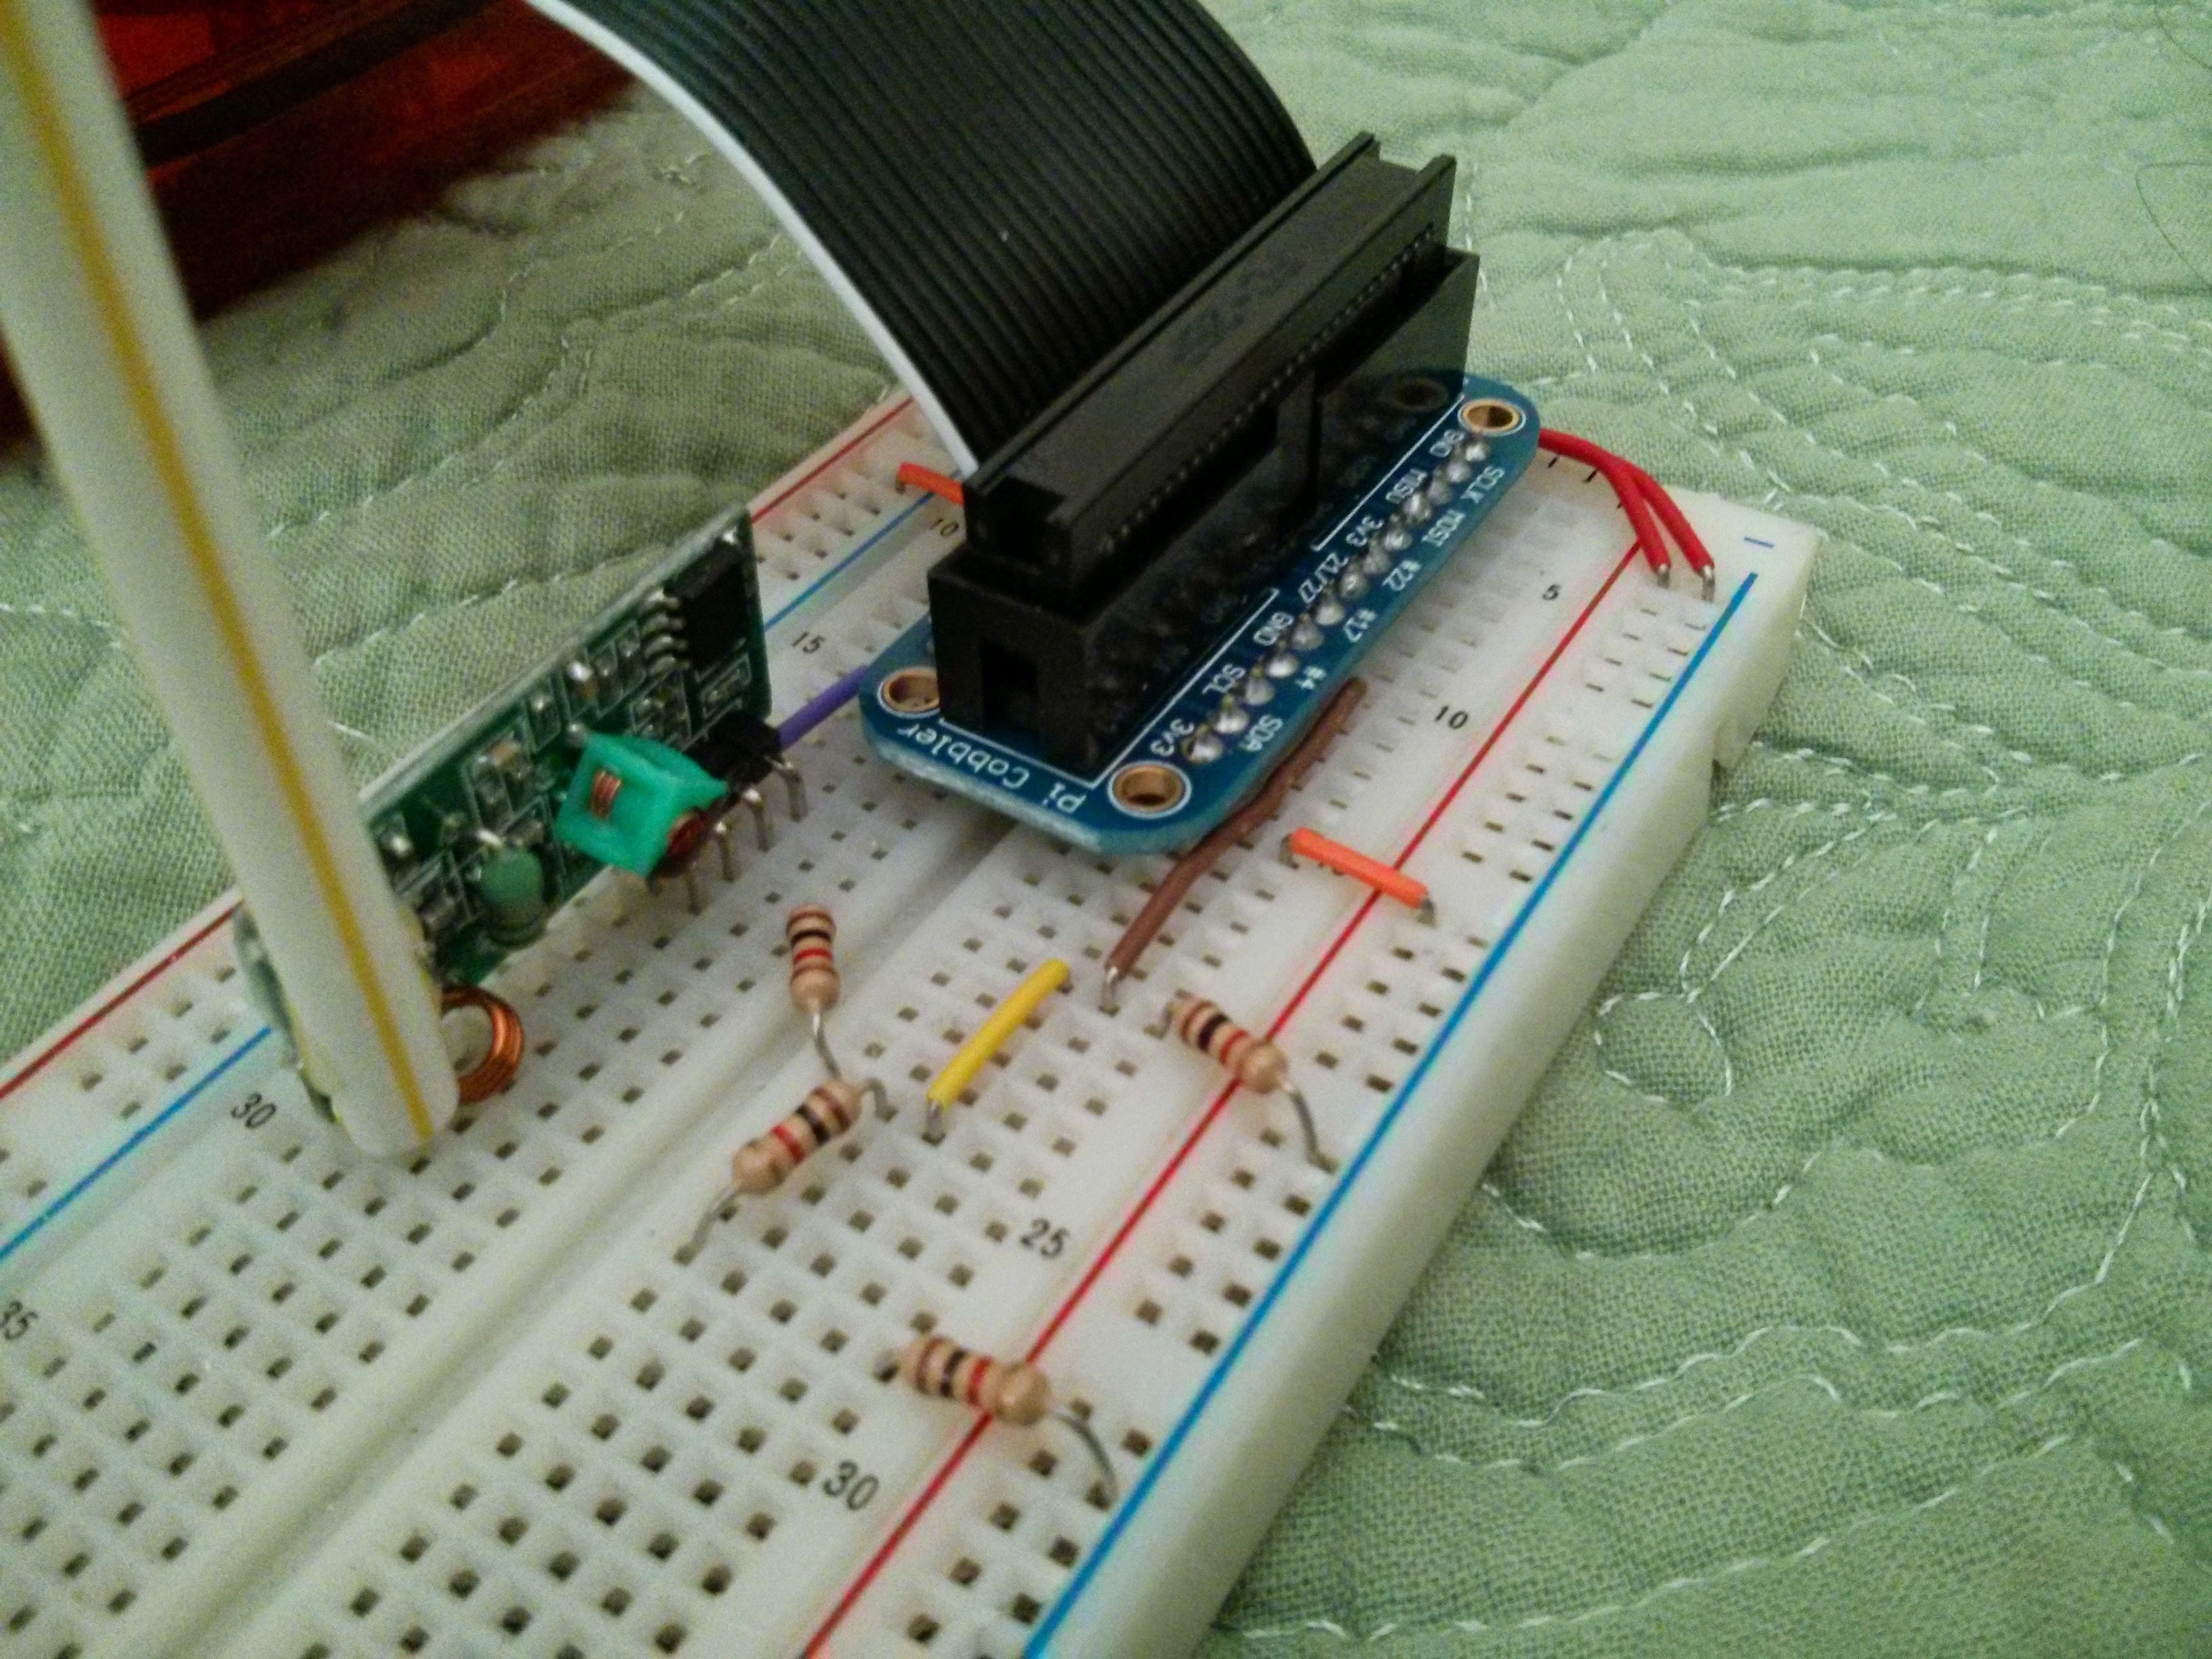
\includegraphics[width=\textwidth]{RaspberryPiRX.jpg}
		\caption{Raspberry Pi RX }
		\label{fig:pirx}
	\end{subfigure}%
	~ %add desired spacing between images, e. g. ~, \quad, \qquad etc.
	%(or a blank line to force the subfigure onto a new line)
	\begin{subfigure}[b]{0.3\textwidth}
		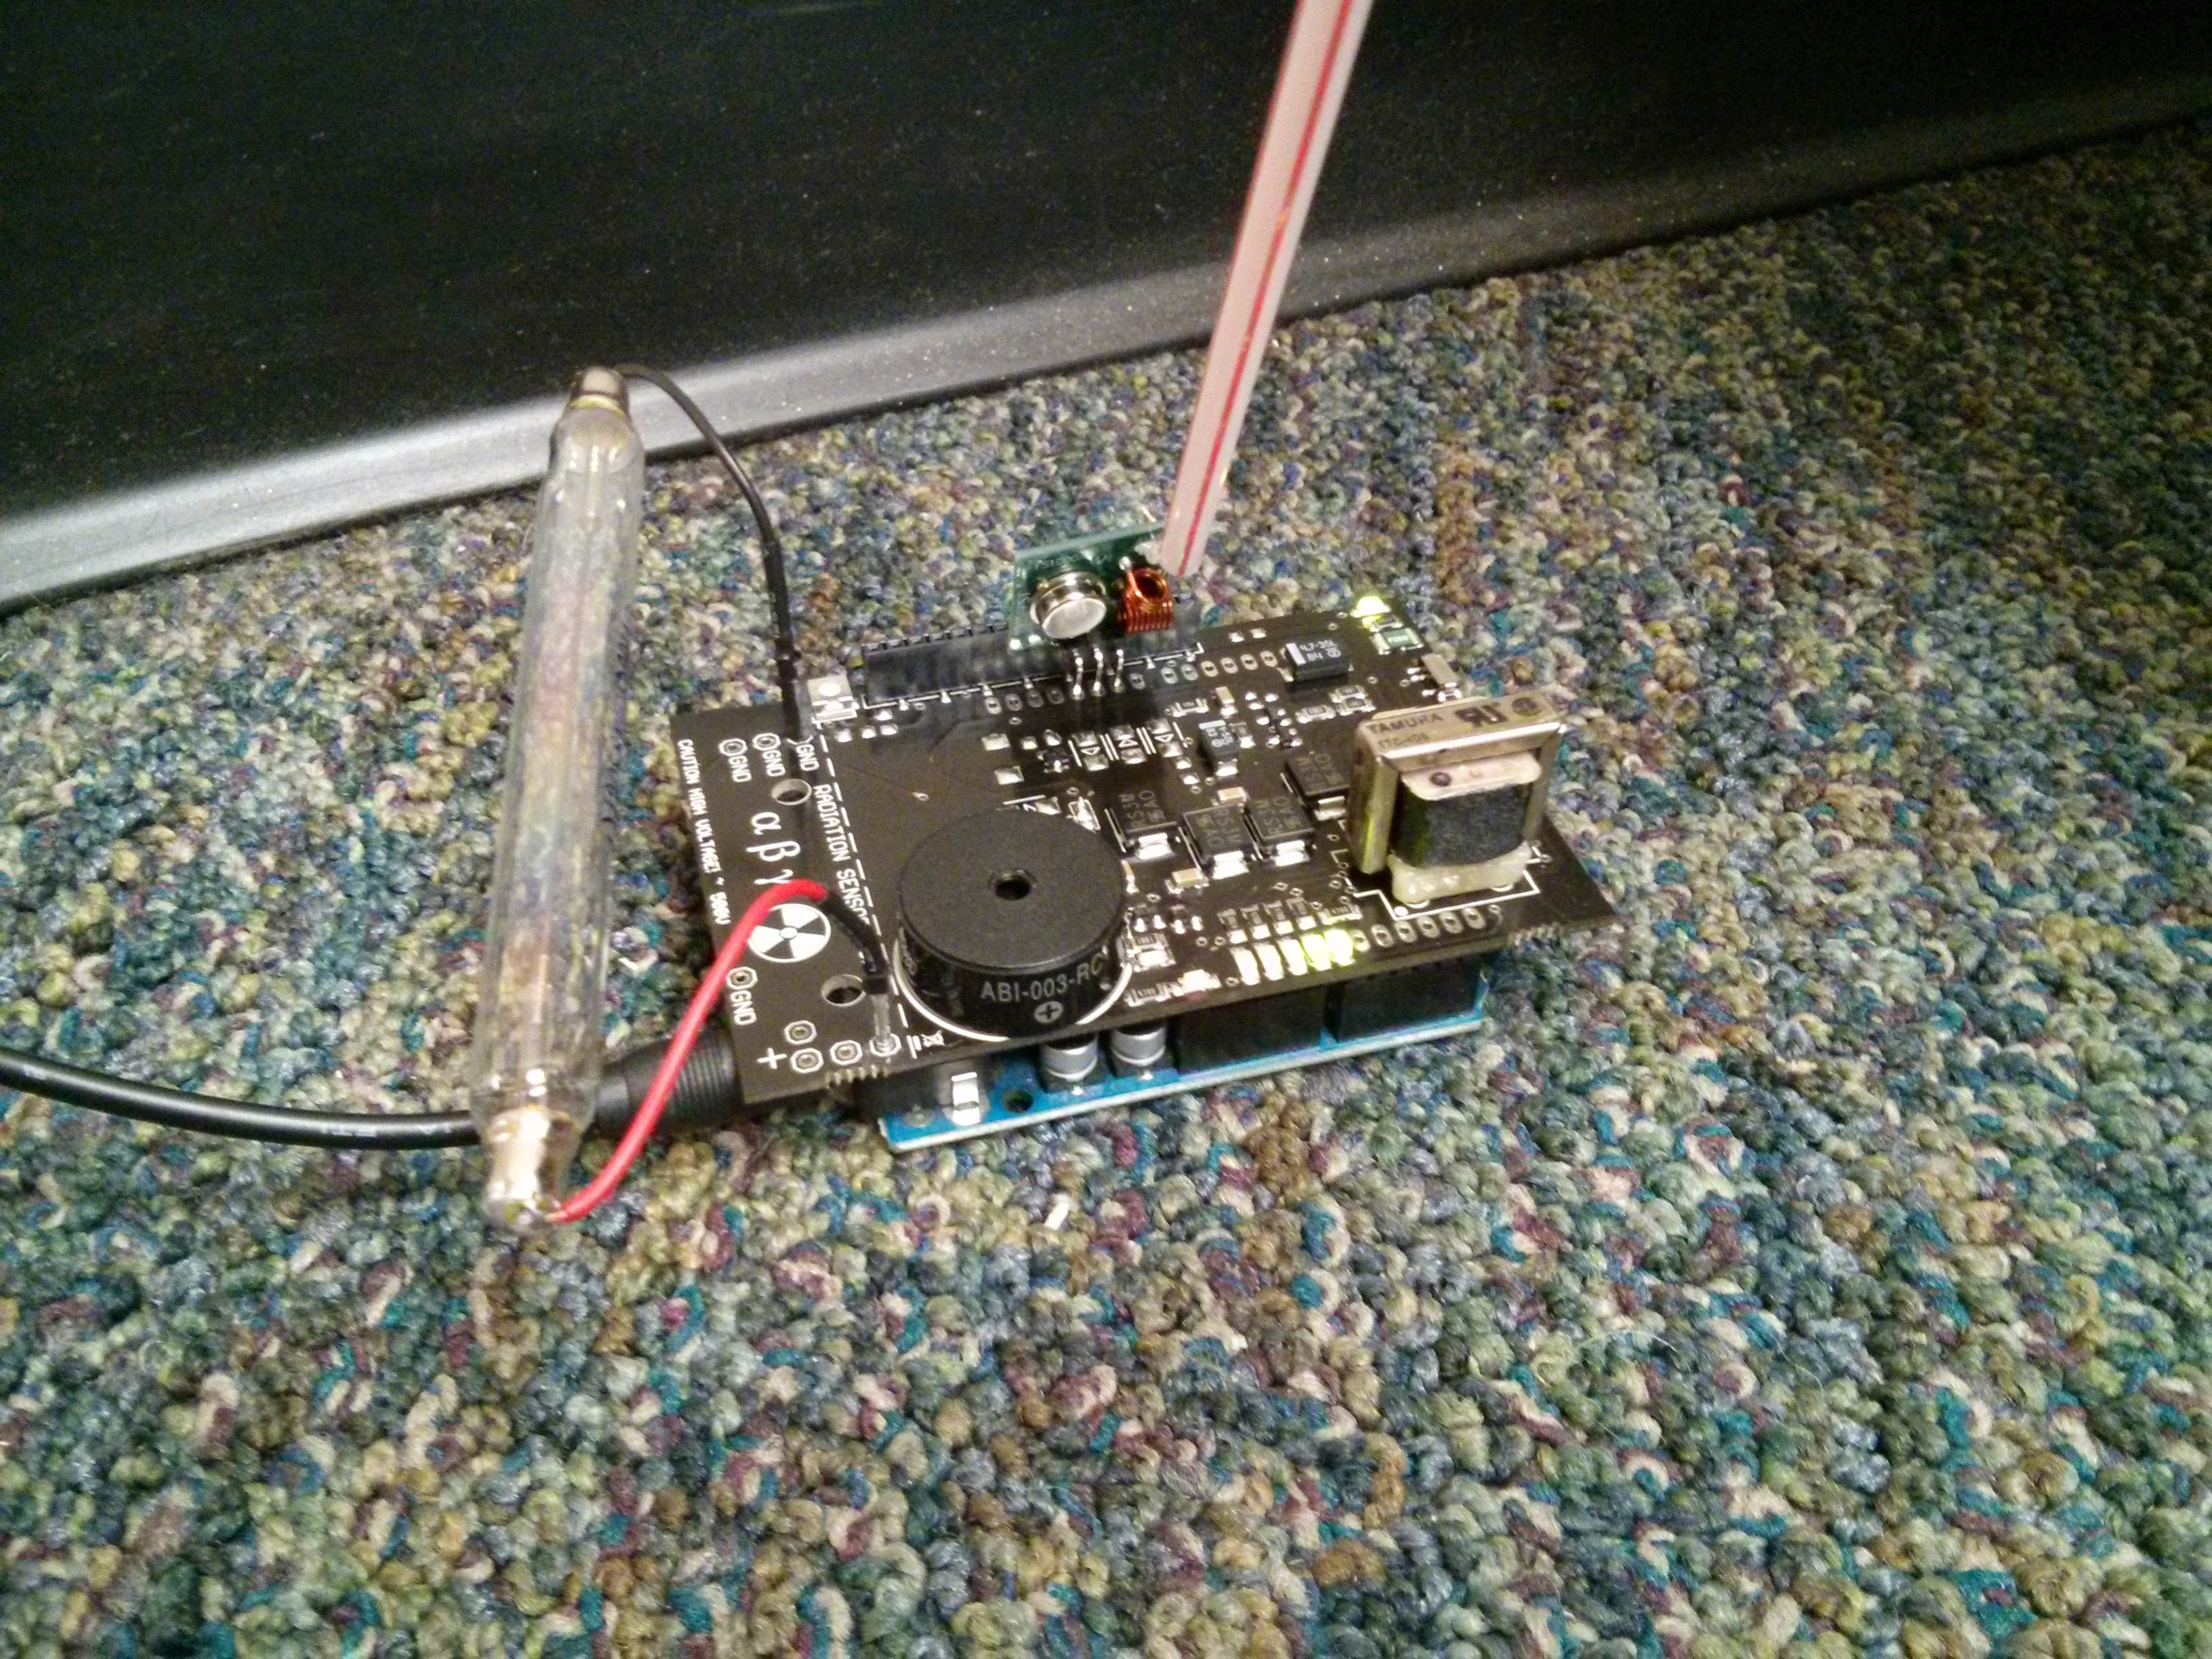
\includegraphics[width=\textwidth]{TransmitterArduinoCarpet.jpg}
		\caption{Arduino Transmitter}
		\label{fig:arduinotx}
	\end{subfigure}

	\caption{Prototype devices}\label{fig:txrx}
\end{figure}

\subparagraph{Power}
The device design has not reached the phase to focus on power consumption. The power regulators on the board consume the majority of power and therefore even an estimation of the final designs power consumption would not be possible. The unit is not able to run for elongated periods of time on batteries, although because the average current consumption is less than 100mA and is dependent on the amount of radiation it could be run from a solar panel.

\subparagraph{Cost}
Although the price per module was not reduced to the expected final product's cost, the device's cost per sensor is lower than commercially available sensors. The cost per module was reduced to about \$130 per transmitter mostly representing the cost of the Arduino Geiger Shield, with the Microcontroller unit and radio transmitter as the rest of the cost.

\subparagraph{Testing Range}
Range tests were conducted of the 433 MHz modules with a 173mm quarter wave whip antenna, with an indoor range of approximately 10m, it can be used in close range, but would fare much better outdoors. With a longer range due to less obstruction, approximately 30m is enough to mount receivers on lamp posts in urban areas, and attach the sensing transmitters to nearby buildings. Testing of multiple devices was also done, the receiver successfully took data from two sensors and differentiated counts based on their address. Through testing, of the 13588 rows transmitted, only 14 were not received properly.

\subparagraph{Server}

The server was built on two platforms based on usage scenarios. The Raspberry Pi (a small, inexpensive ARM based computer), and a Arduio. The Raspberry Pi also has the advantage of not needing anything but a 700mA power connector and an Ethernet port. This server is able to provide live data through a web page and internally through a SQL query-able database shown in Figure~\ref{webPage}. The Arduino based implementation (Figure~\ref{arduinorx}) is great for debugging and testing transmitter technologies before they need to be ported.

\begin{figure}[h]
	\centering
	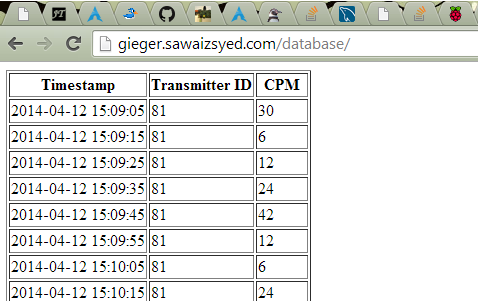
\includegraphics[width=0.5\textwidth]{WebDatabase.png}
	\caption{Web Page hosted on Raspberry Pi \label{webPage}}
\end{figure}

\begin{figure}[h]
	\centering
	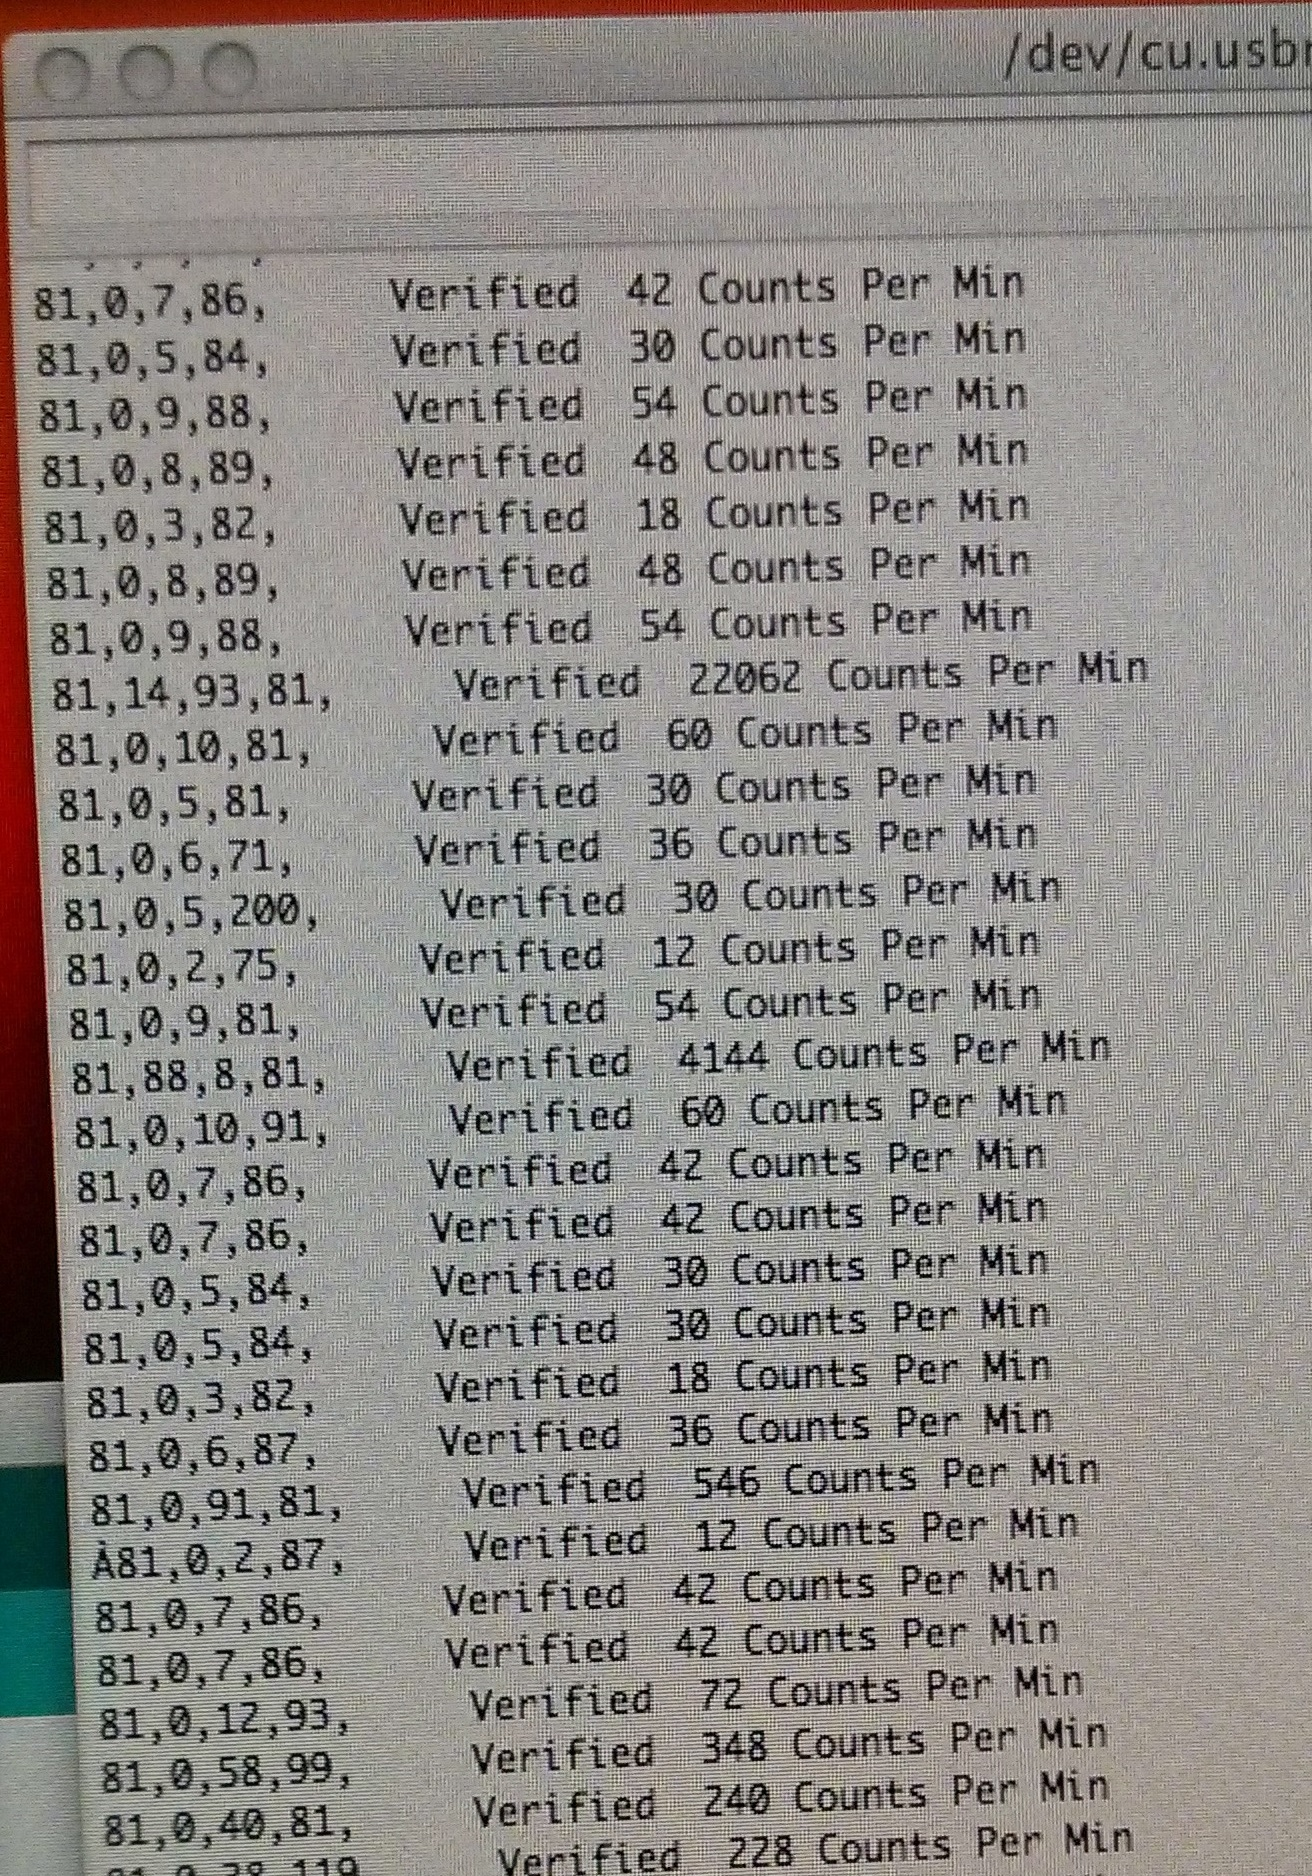
\includegraphics[width=0.5\textwidth]{ArduinoRX}
	\caption{Arduino Receiving Data \label{arduinorx}}
\end{figure}

\subparagraph{Documentation}
All the hardware and software specifications to this point are hosted on-line under open source licenses. There is also documentation of hardware setups and code hosted on an internal Wiki for parallel testing. This documentation allows upkeep of the code-base and devices by others.

\subsection*{Future Prospects}
The device still has a lot to be completed before it reaches the production quality needed. The prototype has shown significant promise and therefore steps to the final product should be few.

\subparagraph{Production}
Preparing the device for production, with custom made circuit boards, and reducing connectors, and part counts is the best way to reduce cost. For this to take place, components need to be ordered an assembled in prototypes of circuit boards and casing.

\subparagraph{Radio Transmitter}

For longer range modules using the NRF24L01+ chip based modules, are available and suggest a more concrete hardware link, and with their engineered antennas, provide longer range.

\pagebreak
\bibliographystyle{plain}
\bibliography{RadiationSensor}

\end{document}